\documentclass[10pt,a4paper]{article}

\usepackage[utf8]{inputenc}
\usepackage[margin=1in]{geometry}
\thispagestyle{empty}

\usepackage{amsmath}
\usepackage{amsfonts}
\usepackage{amssymb}

\usepackage{parskip}

\usepackage{listings}
\usepackage{xcolor}

\usepackage{enumerate}

\usepackage{hyperref}

\usepackage{float}
\restylefloat{figure}
\usepackage[font=small,labelfont=bf]{caption}
\usepackage{wrapfig}

\usepackage{graphicx}
\restylefloat{figure}

\usepackage{cancel}

\usepackage{multicol}
\setlength{\columnsep}{22pt}

\usepackage{colortbl}

\usepackage{cases}

\title{Redes y Comunicaciones de Datos I}
\author{Resumen}

\begin{document}
\maketitle

\section{Conceptos Básicos}

\textit{Telemática}: ciencia que utiliza las telecomunicaciones para potenciar las posibilidades y aplicaciones de la informática.

\subsection{Arquitectura de Redes}
\begin{description}
\item \textbf{Redes de computadoras.} Conjunto de computadoras autónomas \textbf{interconectadas}.

Dos computadoras están \textit{interconectadas} cuando pueden intercambiar información, servicios, recursos, etc. Esta interconexión puede realizarse a través de distintos medios, como ser \textit{cables de cobre, fibra óptica, microondas, rayos infrarrojos, satélites, etc}. 

\item \textbf{Sistemas distribuidos.} Un conjunto de computadoras independientes aparece ante sus usuarios como un sistema consistente y único.
\end{description}
La diferencia entre ambas está en el \textbf{software} (en el SO sobretodo), más que en el \textbf{hardware}.

\subsection{Dispositivos utilizados para la interconexión de Redes}

\begin{itemize}
\item \textit{Repetidores} (regeneran la señal) y \textit{amplificadores} (la amplifican).
\item \textit{Puentes} (Bridges).
\item \textit{Conmutador o Router}: Dispositivo especializado en la conmutación de paquetes. Generalmente utiliza un hardware y software diseñados a propósito.
\item \textit{Gateway}.
\end{itemize}

\subsection{Clasificación de las Redes}
\subsubsection{Según tecnología de transmisión}
\begin{description}
\item \textbf{Enlaces de difusión} (\textit{redes broadcast).} Estas redes tienen un solo canal de comunicación por lo que todas las máquinas de la red lo comparten; si una máquina envía un \textbf{paquete}, todas las demás lo reciben. Cuando las máquinas reciben un paquete verifican la dirección de destino (guardada dentro del paquete) y solo el destinatario lo procesara, los demás lo desecharán. ``\textit{La información se envía a todos los nodos de la red, aunque solo interese a unos pocos}''.

Estos sistemas soportan también el envío de paquetes con una dirección de difusión (\textit{broadcast}) en el destinatario, en este caso todos los que reciben el paquete lo procesaran. Por último puede enviarse un paquete a un conjunto de máquinas, esto se conoce como multidifusión (\textit{multicasting}).

Se pueden crear \textbf{redes planas}, es decir redes en las que la comunicación entre dos ordenadores cualesquiera se haga de forma directa, sin routers intermedios. Presenta posibles problemas de seguridad.

\item \textbf{Enlaces punto a punto.} Estas redes constan de muchas conexiones entre pares individuales de máquinas. Para ir del origen al destino, un paquete en este tipo de red podría tener que visitar primero a una o varias máquinas intermedias. El transporte de datos en estas redes se conoce como unidifusión (\textit{unicasting}). ``\textit{La información se envía solo al nodo al cual va dirigida}''.

Generalmente la comunicación entre dos ordenadores cualesquiera se realiza a través de nodos intermedios que \textbf{encaminan} o \textbf{conmutan} los paquetes. En un enlace punto a punto, el conjunto de router o conmutadores y los enlaces que los unen forman lo que se conoce como \textbf{subred}.

Además, permite crear topologías complejas (\textit{anillo, malla, estrella, etc}).

Los enlaces pueden ser:
\subitem + \textbf{Simplex:} transmisión en un solo sentido.
\subitem + \textbf{Half-duplex:} transmisión en ambos sentidos, pero no a la vez.
\subitem + \textbf{Full-duplex:} transmisión simultánea en ambos sentidos.

En el caso de \textit{full-duplex} y \textit{half-duplex} el enlace puede ser simétrico -misma velocidad en ambos sentidos- o asimétrico. Normalmente, los primeros son simétricos.
\end{description}
\textit{Nota:} Las redes de poca cobertura geográfica tienden a utilizar la \textit{difusión}, mientras que las de cobertura más grande usan la \textit{punto a punto}.

\begin{figure}[ht!]
  \caption{Topologías LAN típicas, izquierda \textbf{bus} (\textit{ethernet}) y derecha \textbf{anillo} (\textit{token ring}).}
  \label{fig:topologia_lan}  
  \centerline{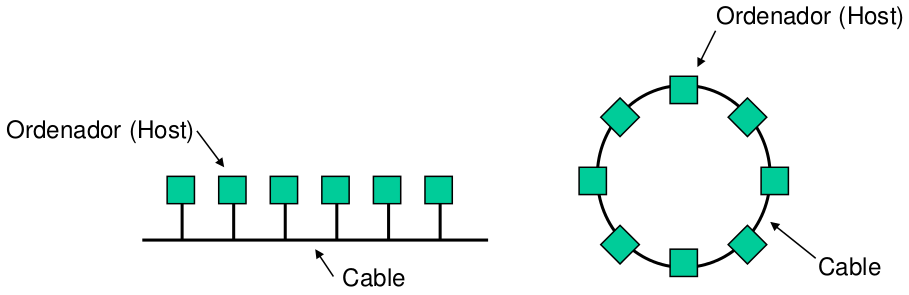
\includegraphics[width=0.7\textwidth-\fboxrule-\fboxrule]{imgs/topologia_lan.png}}  
\end{figure}

\subsubsection{Según su cobertura geográfica}

\begin{description}
\item \textbf{PAN} (\textit{$\approx 1$ metro}). Destinadas a una sóla persona.

\textit{Ejemplo}: una red que conecta los distintos dispositivos de una computadora.
\item \textbf{LAN} (\textit{$\leq 1$ km}). Redes privadas cuyo ámbito no sobrepasa un edificio o campus. Se caracterizan por su alcance, tecnología de transmisión (generalmente \textit{broadcast}), y topología. Están diseñadas desde el principio para transportar datos. El cableado es propiedad del usuario normalmente.

\textit{Ejemplos}: ethernet, token ring, redes inalámbricas por radio.

\item \textbf{MAN} ($\leq 10$ \textit{km}). Abarca una ciudad.

\textit{Ejemplo:} Red de televisión por cable disponible en muchas ciudades.

\item \textbf{WAN} ($\leq 1000$ \textit{km}). Tienen velocidades de transferencia de datos menores a las LANs. Utilizan la base del sistema telefónico, diseñado inicialmente para transportar voz. Son servicios contratados generalmente a operadoras. Suelen utilizar enlaces \textbf{punto a punto} \textit{temporales} o \textit{permanentes}, salvo las comunicaciones vía satélite que son \textit{broadcast}. Tienen un costo elevado, por lo que se suele optimizar su diseño.
\end{description}

\begin{figure}[ht!]
  \caption{Escenario típico de una red completa.}
  \label{fig:escenario_lan_wan}  
  \centerline{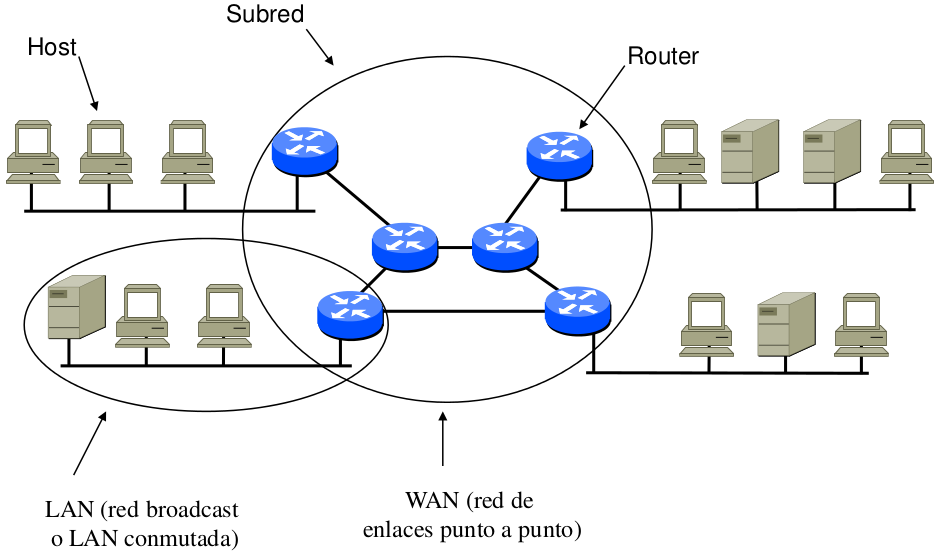
\includegraphics[width=0.7\textwidth-\fboxrule-\fboxrule]{imgs/escenario_lan_wan.png}}  
\end{figure}

\section{Software de Redes}

La interconexión de computadoras es un problema técnico de complejidad elevada y la mejor forma de resolver un problema complejo es dividirlo en partes. En telemática dichas partes se llaman \textbf{capas}, que tienen funciones bien definidas, y están construidas una encima de la otra. El propósito de cada capa es ofrecer ciertos servicios a las capas superiores, a las cuales no se le muestran los detalles de implementación de los servicios ofrecidos.

\subsection{Modelo de Capas}
Actualmente todas las \textit{arquitecturas de red} se describen utilizando un \textbf{modelo de capas}, que permite describir el funcionamiento de las redes de forma modular y hacer cambios de manera sencilla.

\subsubsection{Conceptos básicos}
\begin{description}
\item \textbf{Servicio.} Conjunto de primitivas (\textbf{operaciones}) que una capa proporciona a la capa que está sobre ella. Este define que operaciones puede realizar la capa en beneficio de sus usuarios, pero no dice nada respecto a su implementación. Se relaciona con la interfaz.
\item \textbf{Protocolo.} Conjunto de reglas que rigen el formato y significado de los paquetes que intercambian las entidades iguales de máquinas diferentes.

Normalmente todo protocolo requiere el envío de algunos mensajes especiales o información de control adicional a la que se transmite. Generalmente esto se hace añadiendo una \textbf{cabecera} (\textit{a veces también una \textbf{cola}}) al paquete a transmitir.

La información de control reduce el caudal útil: supone un \textbf{overhead} (\textit{ejemplo}: si tengo un overhead del $20\%$, y tengo que transmitir $100$ \textit{bytes}, en realidad transmito $120$ \textit{bytes}). Como cada capa añade su propia información de control, también añade entonces más \textit{overhead}.

\item \textbf{Interfaz.} Define que operaciones y servicios primitivos pone la capa más baja a disposición de la capa superior inmediata. Si están bien definidas, simplifican el reemplazo de la implementación de una capa por otra implementación totalmente diferente, siempre que se mantengan exactamente los mismos servicios ofrecidos a la capa superior en ambas implementaciones.
\end{description}

Los datos no se transfieren de manera directa de la capa $n$ de una máquina a la capa $n$ de la otra máquina, sino que cada capa pasa los datos y la información de control a la capa inmediatamente inferior, hasta alcanzar la capa más bajo. Debajo de la \textit{capa 1} se encuentra el \textbf{medio físico} a través del cual ocurre la comunicación real.

Un conjunto de capas y protocolos se conoce como \textbf{arquitectura de red}. Ni los detalles de la implementación ni las especificaciones de las interfaces son parte de esta, ya que están ocultas en el interior de la máquina. La lista de protocolos utilizados por un sistema, un protocolo por capa, se conoce como \textbf{pila de protocolos}.

\subsubsection{Objetivos Fundamentales}
\begin{itemize}
\item \textbf{Sencillez}: Hace abordable el complejo problema de la comunicación entre ordenadores.
\item \textbf{Modularidad}: Permite realizar cambios relativamente fáciles a alguna de sus partes sin afectar al resto.
\item \textbf{Compatibilidad}: La comunicación entre dos entidades de una capa puede realizarse independientemente de las demás.
\end{itemize}

\subsubsection{Principios}
\begin{itemize}
\item La capa $n$ ofrece sus servicios a la capa $n+1$.
\item La capa $n+1$ solo usa los servicios de la capa $n$.
\item La capa $n$ solo habla con la capa $n$ de otro sistema (\textit{peer to peer}, ó comunicación igual a igual) siguiendo el protocolo de la capa $n$.
\end{itemize}

\subsubsection{Servicios Orientados a la Conexión y No Orientados a la Conexión}

Las capas pueden ofrecer estos dos tipos de servicios a las capas que están sobre ellas.
\begin{description}
\item \textbf{Orientado a Conexión.} Se concibió en base al sistema telefónico: el usuario del servicio primero establece una conexión, la utiliza, y luego la abandona.

\textit{Características:} Se respeta el orden de los paquetes. Se mantiene la misma ruta o camino para todos los paquetes. Si el canal se corta la comunicación se interrumpe.

\textit{Ejemplos:} red telefónica conmutada, ATM, frame relay.
\item \textbf{No Orientado a Conexión.} Se concibió en base al sistema postal: cada mensaje lleva completa la dirección de destino y cada uno se enruta a través del sistema, independientemente de los demás.

\textit{Características:} No se respeta el orden de los paquetes. La ruta puede variar para cada paquete. La red es más robusta ya que si una ruta queda inservible, pueden usarse otras. Si la comunicación  no es posible los datos se pierden.

\textit{Ejemplos:} IP, ethernet.
\end{description}

\subsubsection{Quality of Service (QoS)}

Consiste en fijar unos valores limites para un conjunto de parámetros (\textit{ancho de banda, latencia, disponibilidad, étc}), asegurando así que la red no se va a congestionar. Se puede ver como una especie de ``\textit{contrato}'' cliente-proveedor.

En un servicio \textbf{confiable} el receptor confirma la recepción de cada mensaje para que el emisor este seguro de que llegó. Como consecuencia de esto hay sobrecargas y retardos que con frecuencia son valiosos pero a veces indeseables. Es por ello que dependiendo de la aplicación, se opta por un servicio \textit{confiable} o no, aunque a veces no está disponible el primero.

\subsection{Modelo OSI}

\subsubsection{Principios}
\begin{itemize}
\item Una capa se debe crear donde se necesite una abstracción bien definida.
\item Cada capa debe realizar una función bien definida.
\item La función de cada capa se debe elegir con la intención de definir protocolos estandarizados internacionalmente.
\item Los limites de las capas se deben elegir a fin de minimizar el flujo de información a través de las interfaces.
\item La cantidad de capas debe ser suficientemente grande para no tener que agrupar funciones distintas en la misma capa y lo bastante pequeña para que la arquitectura no se vuelva inmanejable.
\end{itemize}

\subsubsection{Capas del OSI}
\begin{description}
\item \textbf{Aplicación:} Ofrece a las aplicaciones la posibilidad de acceder a los servicios de las demás capas y define los protocolos que utilizan las aplicaciones para intercambiar datos. El usuario normalmente no interactúa directamente con el nivel de aplicación. Suele interactuar con programas que a su vez interactúan con el nivel de aplicación pero ocultando la complejidad subyacente.
\item \textbf{Presentación:} Encargada de la sintaxis de los datos. Convierte los datos de la red a los datos requeridos por la aplicación.
\item \textbf{Sesión:} Sincroniza el intercambio de datos entre capas inferiores y superiores.
\item \textbf{Transporte:} Esta capa se encarga de que los datos enviados y recibidos lleguen en orden, sin duplicar y sin errores. Puede ser orientado o no a la conexión.
\item \textbf{Red:} Se encarga de enlazar con la red y encaminar los datos hacia sus lugares o direcciones de destino. Brinda la información de hacia dónde debo ir. Esta y las dos capas inferiores se encargan de todo el proceso externo al propio sistema y que están tanto en terminales como en enlaces o repetidores.
\item \textbf{Enlace de datos:} Se encarga de que los datos se envíen con seguridad a su destino y libre de errores. Cuando la conexión no es punto a punto, esta capa no puede asegurar su cometido sino la capa superior. Tiene el control de la capa física.
\item \textbf{Física:} Transmite los datos y suministra servicios a la siguiente capa. Para ello debe conocer las características mecánicas, eléctricas, funcionales y de procedimiento de las líneas.
\end{description}

\subsection{Modelo TCP/IP e Híbrido}

\begin{wrapfigure}[11]{r}{0.45\textwidth}
  \caption{Protocolos y redes del modelo TCP/IP inicial.}
  \label{fig:tcp_ip}  
  \centering
  \hbox{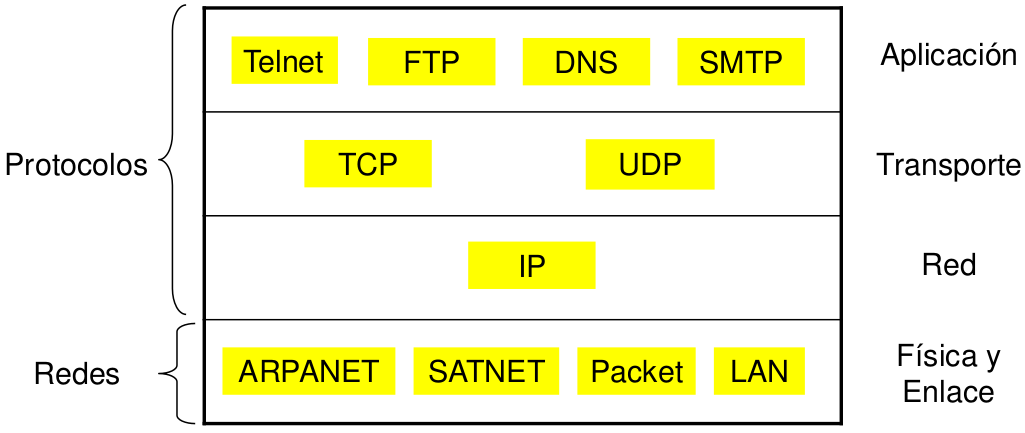
\includegraphics[width=0.45\textwidth-\fboxrule-\fboxrule]{imgs/tcp_ip.png}}  
\end{wrapfigure}

Los protocolos \textbf{TCP/IP} nacieron por la necesidad de ínter-operar redes diversas (\textit{inter-networking}). Se diseño después de los protocolos, por eso a diferencia del \textit{modelo OSI} este tiene protocolos ``predefinidos''. No funciona con otra pila de protocolos.

Cuando se usa un modelo siguiendo el OSI en las capas bajas y el TCP/IP en las altas, se dice que se utiliza un modelo \textbf{híbrido}.

La descomposición del problema de la comunicación en capas es similar que en el OSI. El problema de OSI es que en una capa, todos los protocolos deben tener un funcionamiento similar además de utilizar las funciones definidas en la capa inferior y de suministrar funciones a la capa superior.

\begin{figure}[ht!]
  \caption{Comparación de los distintos modelos.}
  \label{fig:comparacion_modelos}  
  \centerline{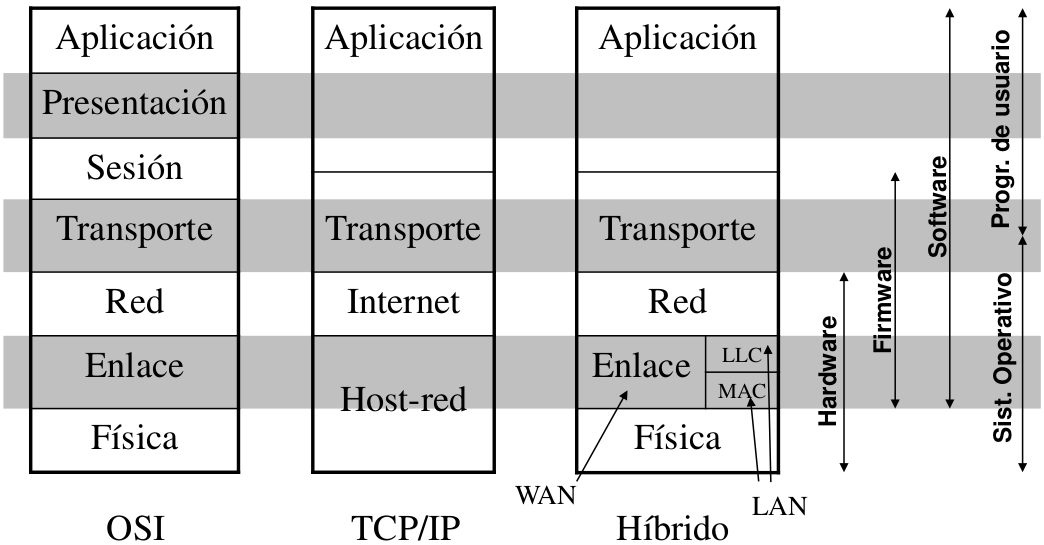
\includegraphics[width=0.8\textwidth-\fboxrule-\fboxrule]{imgs/comparacion_modelos.png}}  
\end{figure}

\subsubsection{Capas de TCP/IP}
\begin{description}
\item \textbf{Aplicación:} proporciona comunicación entre procesos o aplicaciones en computadores distintos.
\item \textbf{Transporte:} encargada de transferir datos ente computadores sin detalles de red pero con mecanismos de seguridad.
\item \textbf{Internet:} se encarga de direccionar y guiar los datos desde el origen al destino a través de la red o redes intermedias.
\item \textbf{Host-Red:} acceso al Medio, asimilable a la capa 2 (enlace de datos) y a la capa 1 (física) del modelo OSI.
\end{description}

\subsubsection{Diferencias entre OSI y TCP/IP}
\begin{itemize}
\item En OSI primero fue el modelo, después los protocolos. En TCP primero los protocolos, después el modelo.
\item En OSI el modelo es bueno, los protocolos malos; en TCP/IP al revés.
\item En OSI los productos llegaban tarde, eran caros y tenían muchas fallas; en TCP/IP todo lo contrario.
\item En TCP/IP los productos aparecían rápido, estaban muy probados (pues los usaba mucha gente), y a menudo eran gratis.
\item OSI soporta comunicación orientada y no orientada a la conexión en la capa de red, pero solo orientada en la capa de transporte; TCP/IP usa un modo no orientado en la capa de red y ambos en la capa de transporte.
\end{itemize}

\subsubsection{OSI modificado}
El que vamos a utilizar. Sus capas son:
\begin{itemize}
\item \textbf{Aplicación} (incluye \textit{sesión} y \textit{presentación}).
\item \textbf{Transporte.}
\item \textbf{Red.}
\item \textbf{Enlace de datos.}
\subitem + Subcapa LLC (\textit{Logical Link Control}).
\subitem + Subcapa MAC (\textit{Media Access Control}).
\item \textbf{Física.}
\end{itemize}

\section{Transmisión de Datos}

\subsection{Conceptos Básicos}
\begin{itemize}
\item \textbf{Dato:} Paquete que vamos a transmitir. Cualquier entidad capaz de transportar información.
\subitem \textbf{+ Analógico:} Datos que pueden tomar valores en un intervalo de tiempo continuo (\textit{ejemplos}: voz, video, temperatura).
\subitem \textbf{+ Digital:} Datos que toman valores discretos (\textit{ejemplos:} cadenas de texto, números enteros).
\item \textbf{Señales:} Representaciones eléctricas o electromagnéticas de los datos.
\subitem \textbf{+ Analógicas:} Onda electromagnética que varía continuamente y que según sea su espectro puede propagarse a través de una serie de medios.
\subitem \textbf{+ Digitales:} Secuencia de pulsos de tensión que pueden transmitirse a través de un medio conductor. Es mas económica que la analógica y menos susceptible al ruido, pero sufre más atenuación.
\item \textbf{Señalización:} Hecho de propagación física de las señales a través de un medio adecuado.
\item \textbf{Transmisión:} Comunicación de datos mediante la propagación y procesamiento de señales.
\subitem \textbf{+ Analógica:} es una forma de transmitir señales analógicas con independencia de su contenido; las señales pueden representar
datos analógicos o datos digitales.
\subitem \textbf{+ Digital:} es dependiente de su contenido. Se puede transmitir a una distancia limitada.
\end{itemize}

\subsection{Transmisión}

\subsubsection{Perturbaciones}
\begin{description}
\item \textbf{Atenuación.} La energía de la señal decae con la distancia por lo que tenemos que asegurarnos que la señal llegue con suficiente energía como para ser captada por la circuitería del receptor, y además el ruido debe ser menor que la señal original. Debido a que la atenuación varía con la frecuencia las señales analógicas llegan distorsionadas por lo que hay que utilizar un sistema que le devuelva sus características iniciales.
\item \textbf{Distorsión de retardo.} Fenómeno debido a que la velocidad de propagación de una señal a través de un medio guiado varía con la frecuencia.
\item \textbf{Ruido.} La señal original resulta modificada debido a distorsiones introducidas por el sistema de transmisión. Es una señal que se inserta entre el emisor y receptor de una señal dada. Hay diferentes tipos de ruido:
\subitem \textbf{+ Ruido térmico:} Ruido que está siempre presente y en todos los dispositivos electrónicos y medios de transmisión. Es función de la temperatura. Cantidad de ruido térmico en un ancho de banda de 1 Hz es: 
$N_0 = KT$ [W/Hz], donde $K = 1.38 \cdot 10^{23} J/$º$K$.
\subitem \textbf{+ Ruido de intermodulación:} Aparecen por un mal funcionamiento del sistema o uso excesivo de energía en la señal.
Es un ruido \textbf{correlacionado} -existe cuando la señal está presente-.
\subitem \textbf{+ Diafonía:} Acoplamiento no deseado de dos o más señales.
\subitem \textbf{+ Ruido impulsivo:} Son pulsos o picos regulares de corta duración y amplitud relativamente grande.
\end{description}

\begin{figure}[ht!]
  \caption{Cuadros comparativos de la transmisión analógica-digital.}
  \label{fig:dig_ana}  
  \centerline{
	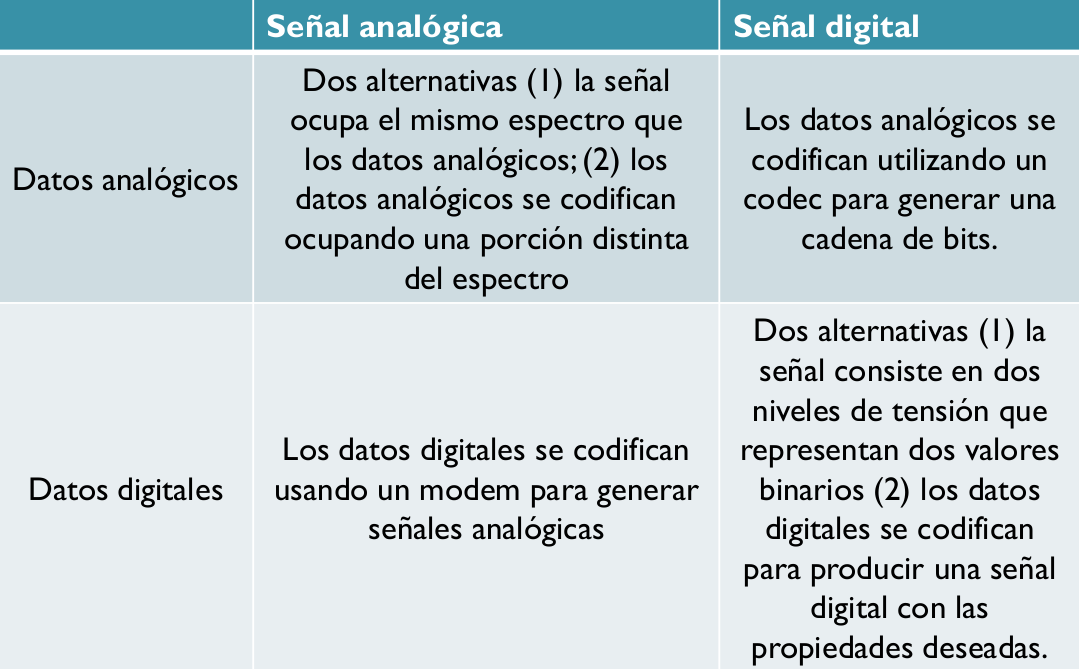
\includegraphics[width=0.75\textwidth-\fboxrule-\fboxrule]{imgs/dig_ana1.png}}
	\vspace{5pt}
  \centerline{
	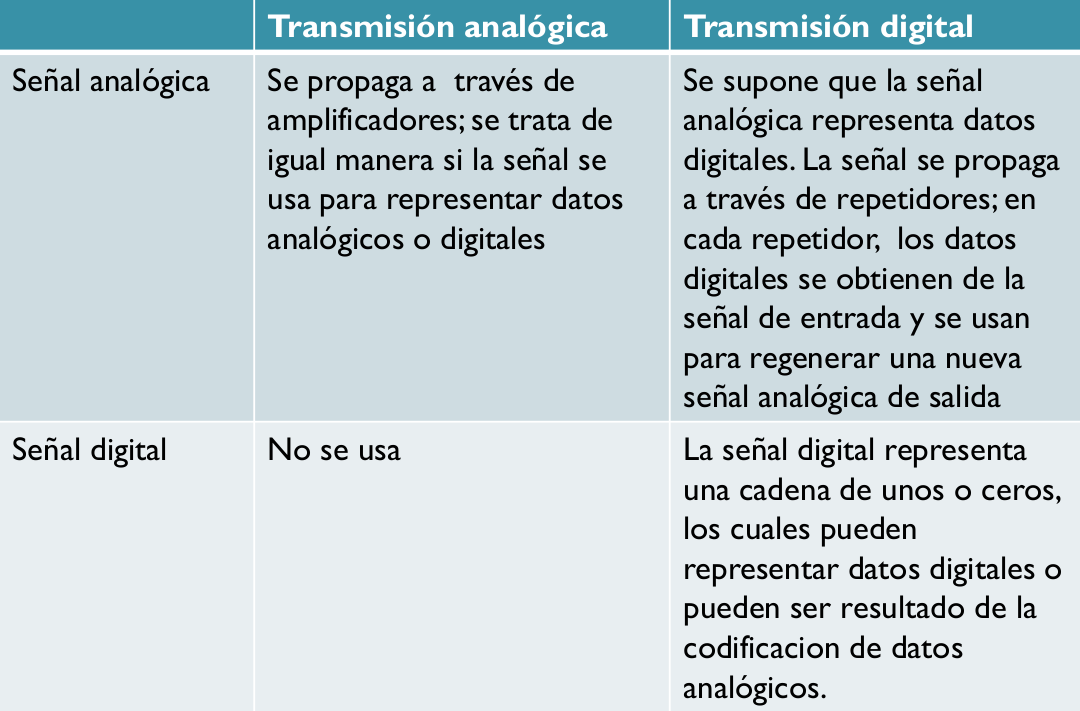
\includegraphics[width=0.75\textwidth-\fboxrule-\fboxrule]{imgs/dig_ana2.png}  
  }  
\end{figure}

\subsubsection{Ventajas de la Transmisión Digital}
\begin{description}
\item \textbf{Tecnología Digital:} más barata y disminuye el tamaño de circuitería.
\item \textbf{Integridad de los datos:} el uso de \textit{repetidores} hace que el ruido y otros efectos no se acumulen. La regeneración de señales mejora el SNR.
\item \textbf{Utilización de la capacidad:} se puede utilizar multiplexación -división en tiempo- de forma más sencilla y de forma más económica.
\item \textbf{Seguridad y Privacidad:} los datos transportados se pueden encriptar.
\item \textbf{Integración:} se procesan tanto datos digitales como analógicos de la misma forma.
\end{description}

\subsubsection{Desventajas de la Transmisión Digital}
\begin{itemize}
\item Transmitir señales analógicas por transmisión digital requiere el uso de mayor ancho de banda, según el teorema de muestreo el doble de frecuencia.
\item Las señales analógicas antes de transmitirse deben transformarse en digitales y luego de nuevo en analógicas antes de ser entregada al emisor. Doble conversión.
\item Requiere sincronización precisa: cuando tengo una cadena de bits de 1 o 0 tengo que determinar cuántos son los bits de esa cadena.
\item En cualquier caso una señal cuando se transmite ira atenuándose con la distancia. Para evitarlo el sistema de transmisión analógica incluye \textit{amplificadores} que inyectan energía, pero introducen ruido. El sistema de transmisión digital, es diferente ya que depende del contenido de la señal y solo puede transmitir en una distancia limitada. Estos incluyen \textit{repetidores}, reciben la señal digital, regeneran el patrón de bits y los retransmite. 
\end{itemize}
\textit{Nota}: si una señal analógica transporta datos digitales se usa repetidores en vez de amplificadores.

\subsection{Relación señal/ruido SNR}
Es la relación que utilizamos para saber cuánto ruido tenemos en nuestra señal de interés. Normalmente la expresamos en dB (\textit{decibeles}). Son valores de \textbf{potencia}, pero también pueden ser representados como valores de tensión o de corriente. \textbf{MAYOR} es el \textbf{SNR}, \textbf{MEJOR} es nuestro sistema de comunicación.

\subsection{Factor de ruido}
Es la relación que existe entre la entrada y la salida de un equipo amplificador: para las señales \textbf{analógicas}, cuando pasa por un \textbf{amplificador} el ruido aumenta.
\[F_\text{ruido} = \frac{\text{SNR (entrada)}}{\text{SNR (salida)}}, \quad \text{con} \quad   F_\text{ruido} \geq 1.\]

\subsection{Capacidad del Canal}
Es la velocidad máxima que se pueden transmitir los datos en un canal de comunicación bajo unos condiciones dadas.

Hay cuatro conceptos en juego relacionados entre sí, que son:
\begin{itemize}
\item \textbf{Velocidad de transmisión:} velocidad, expresada en \textit{bits por segundo} (bps), a la que se pueden transmitir los datos.
\item El \textbf{ancho de banda} estará limitado por el transmisor y por la naturaleza del medio de transmisión; se mide en hercios o ciclos por segundo.
\item \textbf{El ruido:} nivel medio de ruido a través del camino de transmisión.
\item \textbf{Tasa de errores:} tasa a la que ocurren los errores. Se considera que ocurrió un error cuando se recibe un 1 habiendo transmitido un 0 o viceversa.
\end{itemize}

\subsubsection{Ancho de Banda de Nysquit}
Nysquit demostró que dado un ancho de banda $B$, la mayor velocidad de transmisión de la señal que se puede conseguir es $2B$, y viceversa. Si las señales a transmitir son binarias, la velocidad de transmisión que se puede conseguir con $B$ Hz es igual a $2B$ bps.

Si tenemos el caso de señales multinivel, la formulación de Nysquit para el cálculo de la capacidad de canal es: $C=2B \log_2 M$, en bps.

Esto es considerando que no hay ruido.

\subsubsection{Fórmula para la capacidad de Shannon}

Dado un nivel de ruido, cuanto mayor es la velocidad de transmisión, mayor es la tasa de errores. Shannon demostró que los canales son ruidosos, por lo tanto, encontró una ecuación que relación la SNR con la cantidad de niveles de modulación: $M_\text{máx}=\sqrt{1+\text{SNR}}$.

Una conclusión de Shannon es que la capacidad \textbf{máxima} del canal \textit{libre de errores}, en bits por segundo, verifica la ecuación:
\[C=2B\log_2(M_\text{máx})=B\log_2(1+\text{SNR}).\]

Cuanto mayor sea el ancho de banda, más ruido se introducirá en el sistema: cuando $B$ aumenta, $\text{SNR}$ disminuye.

\section{Medios de transmisión}

Es el camino físico entre el transmisor y el receptor. Este medio puede ser:
\begin{description}
\item \textbf{Guiado:} las ondas electromagnéticas se transmiten a través de un medio sólido (\textit{tangible}). Las limitaciones en la transmisión están impuestas por el medio.
\item \textbf{No guiado:} la transmisión inalámbrica se realiza a través de la atmósfera (\textit{intangible}). Las características de la transmisión están más determinadas por el ancho de banda de la señal emitida por la antena que el propio medio.
\end{description}

Hay una serie de factores relaciones con el medio de transmisión y con la señal que determinan tanto la distancia como la velocidad de transmisión:
\begin{itemize}
\item \textbf{El ancho de banda:} al aumentar, la velocidad de transmisión puede incrementar.
\item \textbf{Dificultades en la transmisión:} limitan la distancia (\textit{ejemplo}: atenuación).
\item \textbf{Interferencias:} pueden distorsionar o destruir la señal.
\item \textbf{Número de receptores:} en enlaces compartidos, cada uno de los conectores puede atenuar y distorsionar la señal.
\end{itemize}

\subsection{Medios Guiados}
La capacidad de transmisión depende drásticamente de la distancia y de si el medio guiado es punto a punto o multipunto.

\begin{figure}[ht!]
  \caption{Características de transmisión de medios guiados punto-a-punto.}
  \label{fig:mediospuntoapunto}  
  \centerline{
	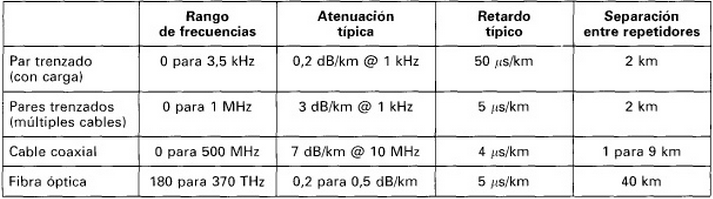
\includegraphics[width=\textwidth-\fboxrule-\fboxrule]{imgs/mediospuntoapunto.png}}
\end{figure}

\subsubsection{Par trenzado}

\begin{figure}[ht!]
  \caption{Características del par trenzado.}
  \label{fig:partrenzado}  
  \centering
  \hbox{
	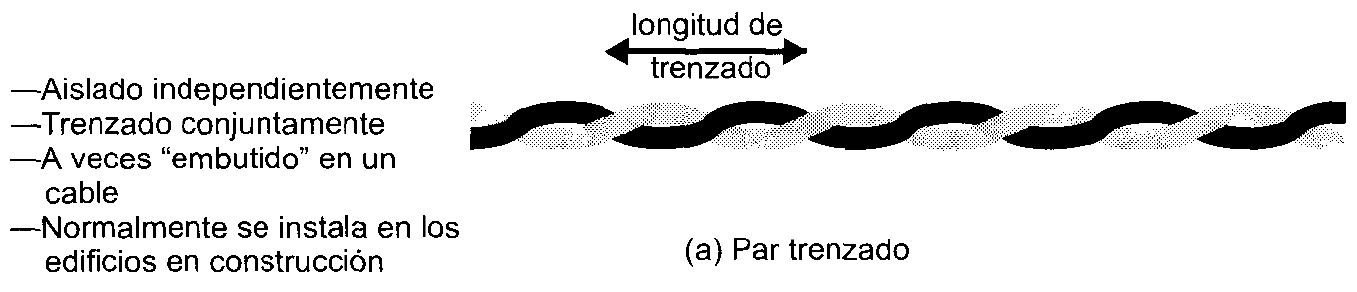
\includegraphics[width=\textwidth-\fboxrule-\fboxrule]{imgs/partrenzado.png}}
\end{figure}

Es el medio de transmisión más usado, el más viejo, el más económico, y el más sencillo de manejar; pero el más limitado en velocidad y distancia máxima. Si la distancia es muy larga, se usan haces (envolturas) que pueden contener cientos de pares (denominados cables multi-pares).

Tiene una fuerte dependencia a la atenuación con la frecuencia. Sirve para transmitir señales tanto analógicas como digitales.

Consiste en dos alambres de cobre aislados de $0.5[mm]$ a $1[mm]$ de espesor. Estos alambres se trenzan en forma helicoidal para evitar la interferencia entre pares (\textit{diafonía}). Existe diafonía en un par trenzado cuando puede medirse una señal que pertenece a otro par cercano. 

Dos parámetros que se miden en par trenzado son el NEXT (\textit{near end crosstalk}), y el FEXT (\textit{far end crosttalk}).

Hay dos variantes de pares trenzados:
\begin{description}
\item \textbf{No apantallado} (UTP, \textit{unshielded twisted pair}): es el menos caro. Es fácil de instalar y de manipular.
\item \textbf{Apantallado}: más difícil y costoso de manipular, pero proporciona mejores prestaciones a altas velocidades de transmisión.
\end{description}

\vspace{10pt}

\textit{Aplicaciones}: Redes de telefonía, redes de comunicación en edificios o campus.

\subsubsection{Cable Coaxial}

\begin{figure}[ht!]
  \caption{Características del Cable Coaxial.}
  \label{fig:cable_coaxial}  
  \centering
  \hbox{
	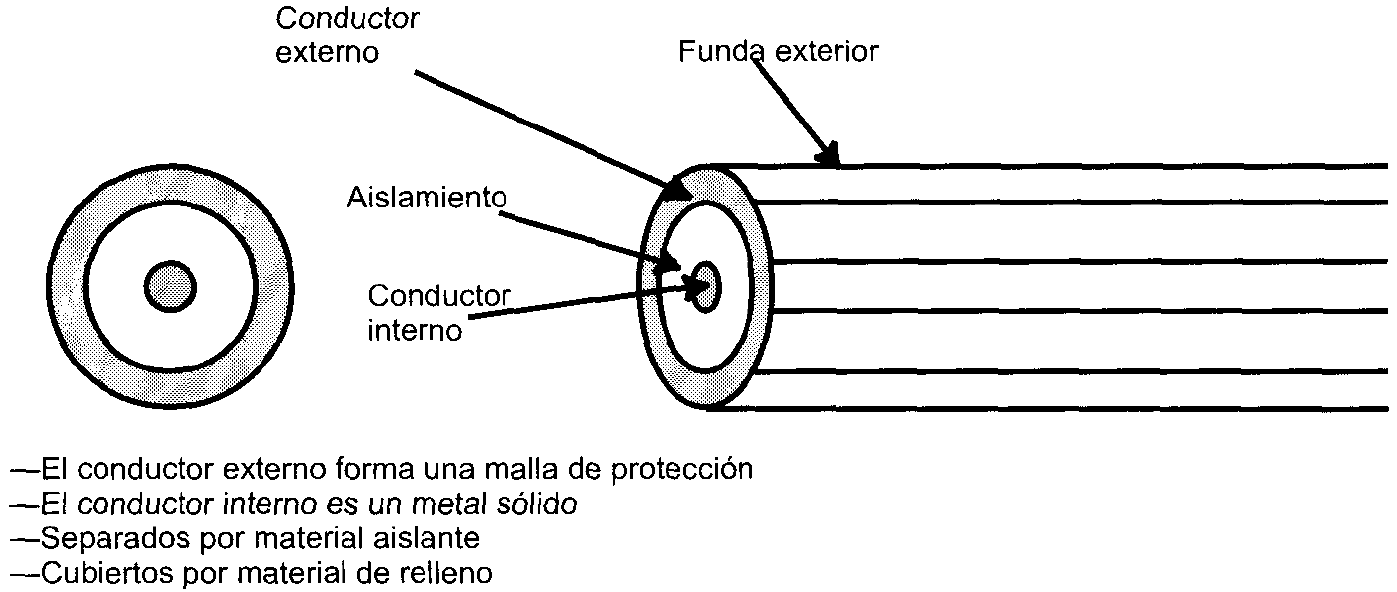
\includegraphics[width=\textwidth-\fboxrule-\fboxrule]{imgs/cable_coaxial.png}}
\end{figure}

\underline{\textbf{Características:}}
\begin{enumerate}[+]
\item Transmite tanto señales analógicas como digitales.
\item Buena respuesta en frecuencia, permitiendo mayores frecuencias y velocidades de transmisión.
\item Por construcción, es menos susceptible a interferencia como a diafonía.
\end{enumerate}

\underline{\textbf{Limitaciones:}}
\begin{enumerate}[+]
\item Atenuación.
\item Ruido de intermodulación y térmico.
\end{enumerate}

\textit{Aplicaciones}: distribución de televisión, telefonía a larga distancia, enlaces en computadoras a corta distancia, LAN.

\subsubsection{Fibra Óptica}

Es un medio flexible y delgado, compuesto por una delgada hebra de vidrio o silicio fundido, capaz de confinar un haz de naturaleza óptica.

\begin{figure}[ht!]
  \caption{Características de la Fibra Óptica.}
  \label{fig:fibra_optica}  
  \centering
  \hbox{
	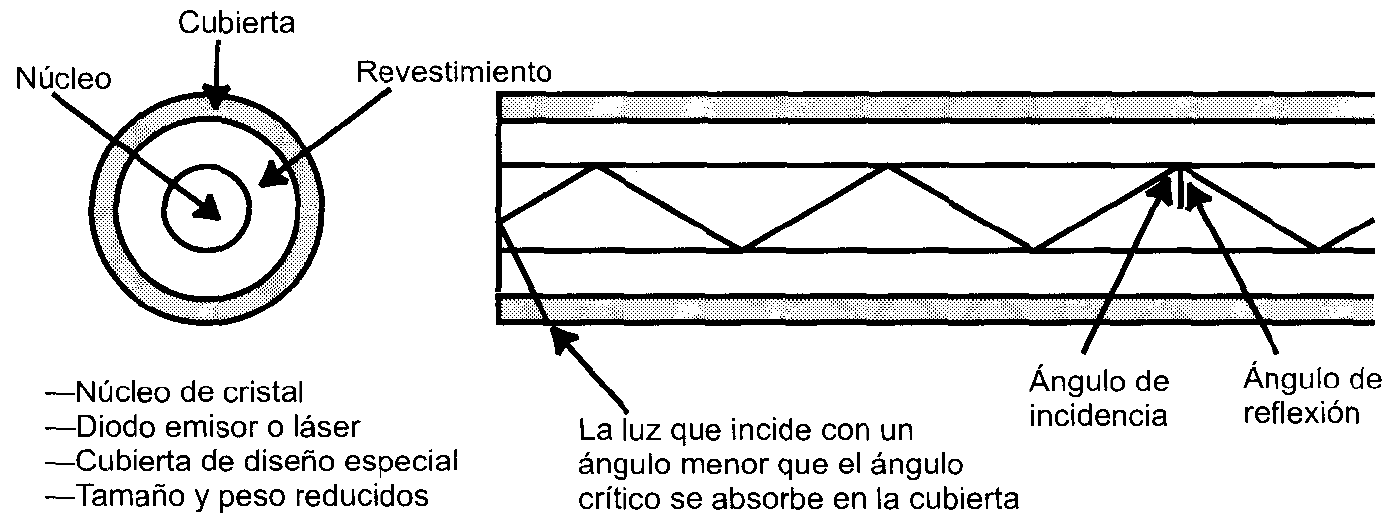
\includegraphics[width=\textwidth-\fboxrule-\fboxrule]{imgs/fibra_optica.png}}
\end{figure}

Hay tres componentes clave por cada filamento: la \textbf{fuente de luz} (LED o Láser), el \textbf{medio transmisor} (la fibra óptica), y el \textbf{detector de luz} (fotodiodo).

\underline{\textbf{Características:}}
\begin{enumerate}[+]
\item \textbf{Mayor Capacidad:} se ha demostrado que se pueden conseguir velocidades de transmisión de cientos Gbps para decenas de kilómetros de distancia.
\item \textbf{Menor tamaño y peso.}
\item \textbf{Atenuación menor.} Además, es constante a lo largo de un gran intervalo.
\item \textbf{Aislamiento electromágnetico:} no se ven afectados por estos campos. No son vulnerables a interferencias, ruido impulsivo, o diafonía. A la vez, sus hebras no irradian energía $\Rightarrow$ no producen interferencias significativas.
\item \textbf{Mayor separación entre repetidores:} menor costo, y menores fuentes de error.
\end{enumerate}

\begin{figure}[ht!]
  \caption{Modos de transmisión en la Fibra Óptica.}
  \label{fig:fibra_optica_modos}  
  \centering
  \hbox{
	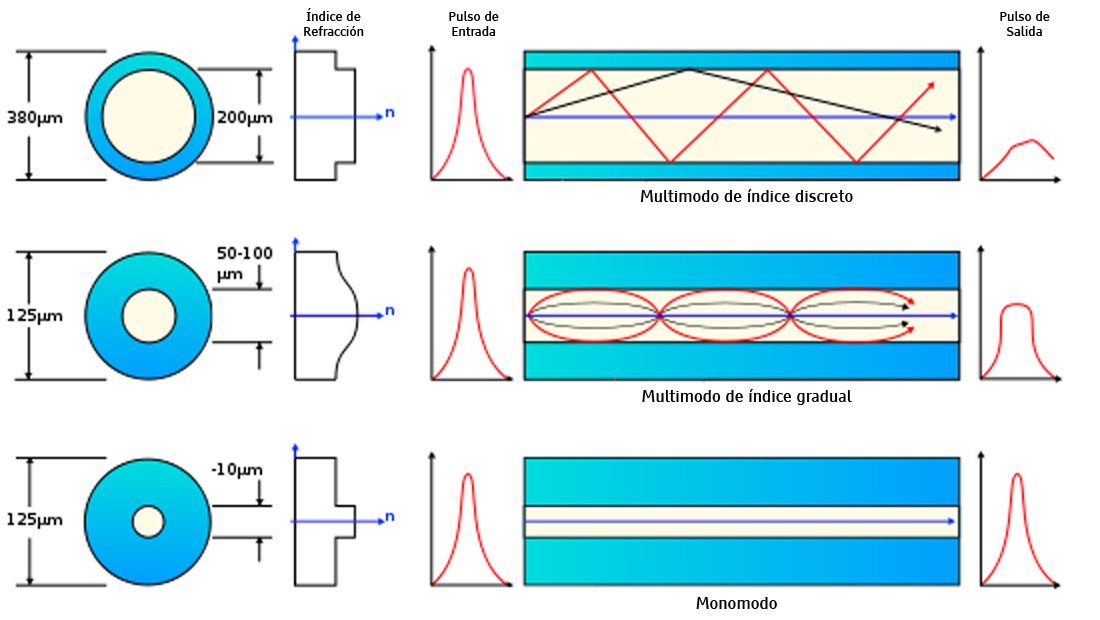
\includegraphics[width=\textwidth-\fboxrule-\fboxrule]{imgs/fibra_optica_modos.png}}
\end{figure}

\vspace{10pt}

\textit{Aplicaciones}: transmisiones a larga distancia y metropolitanas, acceso a áreas rurales, bucles de abonado, LAN.

\underline{\textbf{Modos de transmisión:}}
\begin{description}
\item \textbf{Multimodo.} Su núcleo tiene un índice de refracción superior, pero del mismo orden de magnitud, que el revestimiento. Debido a su gran tamaño, es más fácil de conectar y tiene una mayor tolerancia a componentes de menor precisión. Pero la necesidad de separar los pulsos de luz limita la velocidad de transmisión.

Dependiendo el tipo de índice de refracción, tenemos dos tipos:
\begin{itemize}
\item \textbf{Índice escalonado:} El núcleo tiene un índice de refracción constante en toda la sección cilíndrica, con alta dispersión modal.
\item \textbf{Índice gradual:} El índice de refracción no es constante, tiene menor dispersión modal y el núcleo se constituye de distintos materiales.
\end{itemize}
\item \textbf{Monomodo.} es una fibra óptica en la que sólo se propaga un modo de luz. Se logra reduciendo el diámetro del núcleo de la fibra hasta un pequeño tamaño ($8.3$ a $10$ micrones) que sólo permite un modo de propagación. Su transmisión es paralela al eje de la fibra. Esto le permite alcanzar grandes distancias (hasta $400 [$Km$]$ como máximo, mediante un láser de alta intensidad) y transmitir elevadas tasas de información (decenas de Gbps).
\end{description}

\underline{\textbf{Pérdida en los cables}}

A la pérdida de potencia a través del medio se conoce como atenuación, es expresada en decibelios, con un valor positivo en dB, y es causada por distintos motivos, como la disminución en el ancho de banda del sistema, velocidad, eficiencia. La fibra \textit{multimodal}, tiene mayor pérdida debido a que la onda luminosa se dispersa por las impurezas. Las principales causas de pérdida en el medio son:
\begin{enumerate}[+]
\item \textbf{Pérdidas por absorción:} Ocurre cuando las impurezas en la fibra absorben la luz, y esta se convierte en energía calorífica; las pérdidas normales van de 1 a 1000 dB/Km.
\item \textbf{Pérdida de Rayleigh:} En el momento de la manufactura de la fibra, existe un momento donde no es líquida ni sólida y la tensión aplicada durante el enfriamiento puede provocar microscópicas irregularidades que se quedan permanentemente; cuando los rayos de luz pasan por la fibra, estos se difractan haciendo que la luz vaya en diferentes direcciones.
\item \textbf{Pérdidas por radiación:} Estas pérdidas se presentan cuando la fibra sufre de dobleces, esto puede ocurrir en la instalación y variación en la trayectoria, cuando se presenta discontinuidad en el medio.
\item \textbf{Pérdidas por acoplamiento:} Las pérdidas por acoplamiento se dan cuando existen uniones de fibra, se deben a problemas de alineamiento.
\item \textbf{Dispersión modal:} Es la diferencia en los tiempos de propagación de los rayos de luz, debido a que siguen rutas distintas.
\item \textbf{Dispersión cromática:} Esta dispersión sólo se observa en las fibras tipo monomodal, ocurre cuando los rayos de luz emitidos por la fuente que se propagan por el medio, no llegan al extremo opuesto en el mismo tiempo; esto se puede solucionar cambiando el emisor fuente.
\end{enumerate}

\underline{\textbf{Reflexión y refracción}}

Los principios básicos de su funcionamiento se justifican aplicando las \textit{leyes de la óptica geométrica}, principalmente, la \textbf{ley de la refracción} (principio de reflexión interna total) y la \textbf{ley de Snell}.

Su funcionamiento se basa en transmitir por el núcleo de la fibra un haz de luz, tal que este no atraviese el revestimiento, sino que se refleje y se siga propagando. Esto se consigue si el \textbf{índice de refracción} del núcleo es mayor al índice de refracción del revestimiento, y también si el \textbf{ángulo de incidencia} es superior al \textbf{ángulo crítico}.

\begin{figure}[ht!]
  \caption{\textbf{(1)} La luz incidente a cualquier ángulo menor que el ángulo critico ($\alpha_1 < \alpha_\text{crítico}$) no se refleja totalmente. Parte de la energía del rayo incidente se refracta; \textbf{(2)} El rayo incidente al emerger lo hace a lo largo de la superficie de separación de los dos medios ($\alpha_2 = \alpha_\text{crítico}$); \textbf{(3)} Ocurre reflexión total interna ($\alpha_3 > \alpha_\text{crítico}$), toda la energía del rayo permanece dentro del ámbito de $n_1$.}
  \label{fig:snell}  
  \centering
  \hbox{
	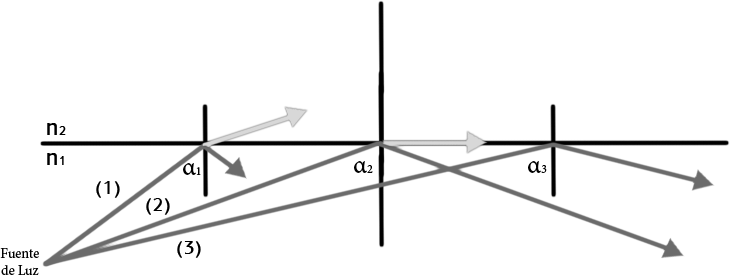
\includegraphics[width=\textwidth-\fboxrule-\fboxrule]{imgs/snell.png}}
\end{figure}

En la \textbf{figura \ref{fig:snell}} podemos ver los distintos casos de rayos incidentes, y cuando se produce la \textbf{reflexión total interna}. La \textbf{Ley de Snell} establece que: 
\[n_1 \sin(\alpha)=n_2 \sin(\beta).\]

\underline{\textbf{Ángulo de aceptación}}

Es el máximo ángulo en el cual los rayos de luz externos pueden chocar con la interfaz revestimiento-fibra y aun propagarse por la fibra con una respuesta no mayor a 10dB de máximo valor. Si giramos el ángulo $\theta_\text{in}$ de aceptación alrededor del eje de la fibra, describe el \textbf{cono de aceptación} de entrada.

\begin{figure}[ht!]
  \caption{Sección lateral de una fibra óptica. Todos los rayos incidentes entre $R_1$ y $R_3$ (dentro del ángulo máximo de aceptación) se propagarán por la fibra.}
  \label{fig:angulo_aceptacion}  
  \centerline{
	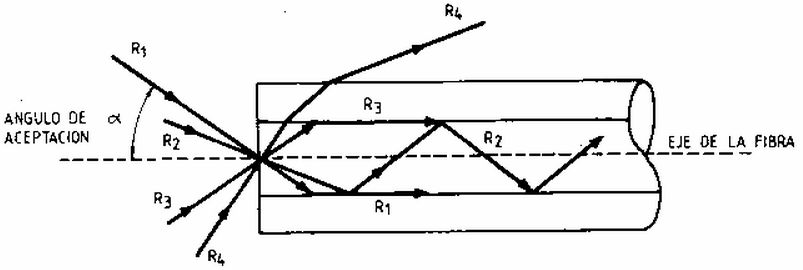
\includegraphics[width=0.9\textwidth-\fboxrule-\fboxrule]{imgs/angulo_aceptacion.png}}
\end{figure}

\underline{\textbf{Cálculo del ángulo de aceptación}}

Cuando los rayos de luz entran en la fibra, chocan con la interfaz de aire/vidrio, en la normal $A$. En consecuencia, la luz que entra en la interfaz de aire vidrio/vidrio se propaga de un medio menos denso a un medio más denso. Esto causa, de acuerdo a la \textit{ley de Snell}, que los rayos de luz cambien de dirección y se propaguen diagonalmente por el núcleo a un ángulo $\theta_c$ que es diferente al ángulo de incidencia externo $\theta_\text{in}$. Para que un rayo pueda propagarse por un cable, debe chocar a la interfaz de núcleo/cubierta interno a un ángulo que sea mayor que el ángulo crítico $\theta_c$.

\begin{figure}[ht!]
  \caption{Propagación del rayo adentro y abajo de un cable de fibra óptica.}
  \label{fig:calculo_angulo_aceptacion}  
  \centering
  \hbox{
	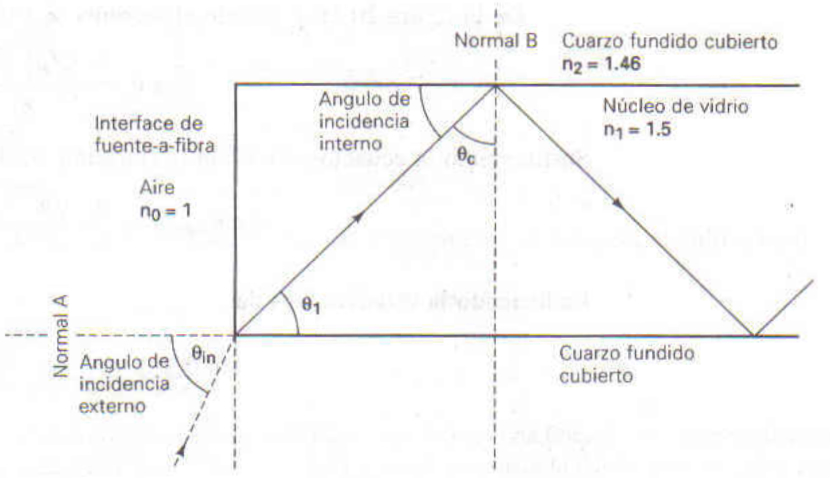
\includegraphics[width=\textwidth-\fboxrule-\fboxrule]{imgs/calculo_angulo_aceptacion.jpg}}
\end{figure}
 
Aplicando la \textit{ley de Snell} a $\theta_in$:
\begin{align*}
n_0 \sin (\theta_\text{in}) &= n_1 sin (\theta_1), 
&\theta_1 = 90 - \theta_c, \\
\sin (\theta_1) &= \sin(90 - \theta_c) = cos (\theta_c), \\
&\Rightarrow n_0 \sin (\theta_\text{in}) = n_1 cos (\theta_c).
\end{align*} 

Rearreglando, y usando el teorema de pitágoras (ver \textbf{figura \ref{fig:pitagoras}}):
\begin{align*}
\sin (\theta_\text{in}) \; \frac{n_1}{n_0} &= \cos(\theta_c), \\
\cos (\theta_c) &= \frac{\sqrt{n_1^2 - n_2^2}}{n_1}, \\
\sin (\theta_\text{in}) &= \frac{n_1}{n_0} \; \frac{\sqrt{n_1^2 - n_2^2}}{n_1}, \\
\sin (\theta_\text{in}) &= \frac{\sqrt{n_1^2 - n_2^2}}{n_0}.
\end{align*}

Dado a que los rayos de luz generalmente entran a la fibra por un medio de aire, $n_0=1$. Entonces, la ecuación final sería:
\[\theta_\text{in (máxima)} = \sin^{-1} \sqrt{n_1^2 - n_2^2}\]

\begin{figure}[ht!]
  \caption{Relación geométrica en la fibra óptica.}
  \label{fig:pitagoras}  
  \centerline{
	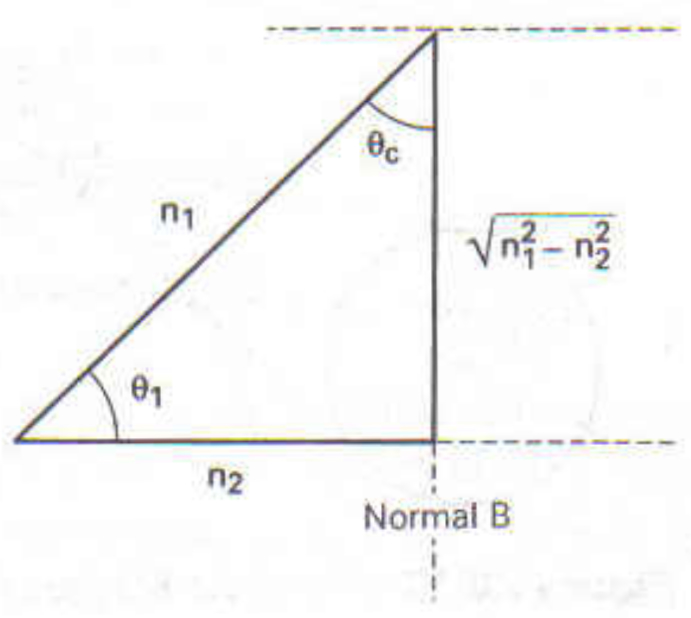
\includegraphics[width=.4\textwidth-\fboxrule-\fboxrule]{imgs/pitagoras.jpg}}
\end{figure}
\pagebreak
\underline{\textbf{Apertura numérica (NA)}}

Describe la habilidad de recojer la luz de una fibra óptica. Entre más grande la magnitud de NA, mayor es la cantidad de luz aceptada por la fibra de la fuente de luz externa. Para una fibra de índice discreto, la NA se define matemáticamente como: $NA = \sin(\theta_{in})$.

\begin{figure}[ht!]
  \caption{Cono de aceptación de una cable de fibra óptica.}
  \label{fig:na}  
  \centerline{
	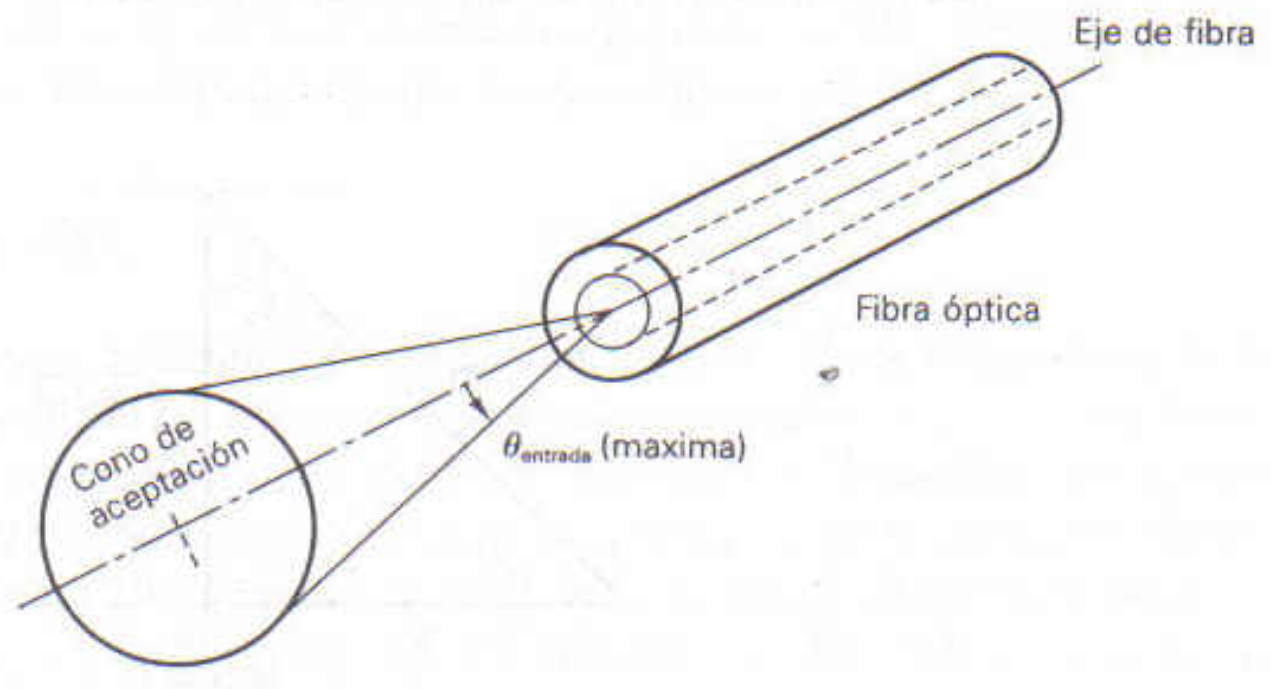
\includegraphics[width=.8\textwidth-\fboxrule-\fboxrule]{imgs/na.png}}
\end{figure}
 
 \pagebreak
\section{Técnicas para la codificación de señales}

\subsection{Conceptos Básicos}
\begin{itemize}
\item \textbf{Señal portadora:} señal continua de frecuencia constante.
\item \textbf{Señal en banda base:} es la señal de entrada que puede ser tanto analógica como digital.
\item \textbf{Modulación:} proceso de codificación de los datos generados por la fuente en la señal portadora de frecuencia $f_c$. Las técnicas de modulación se basan en la modificación de uno o más parámetros fundamentales: \textbf{amplitud, frecuencia, fase}.
\item \textbf{Velocidad de modulación:} velocidad a la que cambia el nivel de la señal, medida en \textit{baudios} (elemento de señal por segundo).
\end{itemize}

\begin{figure}[ht!]
  \caption{Codificación sobre una señal digital (\textit{arriba}); modulación sobre una señal analógica (\textit{abajo}).}
  \label{fig:tecnicas}  
  \centering
  \hbox{
	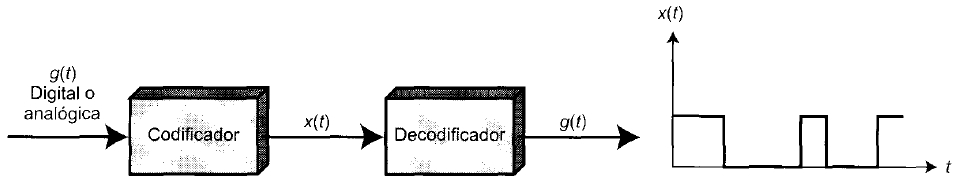
\includegraphics[width=\textwidth-\fboxrule-\fboxrule]{imgs/tecnicas_up.jpg}}
  \hbox{
	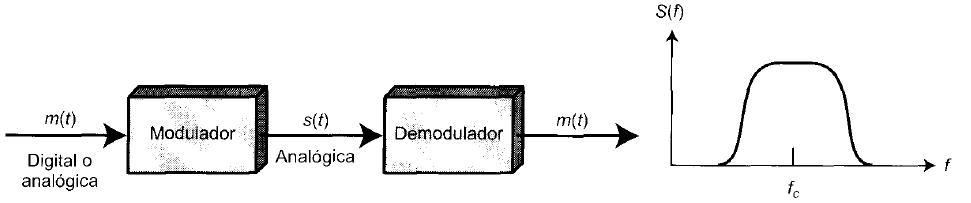
\includegraphics[width=\textwidth-\fboxrule-\fboxrule]{imgs/tecnicas_down.jpg}}	
\end{figure}

\subsection{Datos Digitales, Señales Digitales}

\subsubsection{Conceptos Básicos}
\begin{itemize}
\item \textbf{Duración de un bit:} es el tiempo empleado en el transmisor para emitir un bit, definido por: $1/R$, con $R$ siendo la velocidad de transmisión.
\item \textbf{Señal unipolar:} si todos los elementos tienen el mismo signo algebraico.
\item \textbf{Señal polar:} si un estado lógico se representa con un nivel positivo de tensión, y el otro mediante un nivel negativo.
\item \textbf{Señal bipolar:} un estado lógico se representa con un valor nulo de tensión y el otro estado lógico se representa en forma alternada por valores de tensión positivos y negativos.
\item \textbf{Retorno a cero:} técnica que se puede aplicar a señales polares, unipolares y bipolares; a mitad del intervalo, el valor cae a cero.
\end{itemize}

El receptor debe conocer o determinar la duración de cada bit, y determinar si el nivel de cada bit es alto (0) o bajo(1). Los factores que determinan el éxito o fracaso del receptor al interpretar la señal son:
\begin{itemize}
\item Un incremento en la \textbf{velocidad de transmisión} aumentará la \textit{tasa de errores por bit} (BER).
\item Un aumento en la relación \textbf{SNR} reduce el BER.
\item Un incremento del \textbf{ancho de banda} permite un aumento de la \textbf{velocidad de transmisión}.
\item Mejorar el \textbf{esquema de codificación} mejora las prestaciones del sistema.
\end{itemize}

A continuación se consideran los factores a tener en cuenta para la evaluación y comparación de los distintos esquemas de codificación:
\begin{description}
\item \textbf{Espectro de la señal:} la ausencia de componentes a altas frecuencias significa que se necesita menos ancho de banda para su transmisión. Si la señal tiene continua, para su transmisión se requiere la existencia de una conexión \textbf{física} directa. En la práctica, es frecuente que la función de transferencia del canal se deteriore en las proximidades de los límites de banda. Por tanto, un buen diseño debería concentrar la potencia transmitidad en la parte central del ancho de banda de la señal transmitida.
\item \textbf{Sincronización:} una solución costosa es usar una señal de reloj externa. Otra alternativa es proporcionar la sincronización mediante la propia señal transmitida.
\item \textbf{Detección de errores:} la detección está al nivel de la capa de \textbf{enlace de datos}, pero es útil hacerlo también en la capa \textbf{física}.
\item \textbf{Inmunidad al ruido e interferencia:} algunos códigos exhiben un comportamiento superior que otros en presencia de ruido.
\item \textbf{Coste y complejidad:} cuanto mayor es la \textbf{velocidad de modulación}, para una velocidad de transmisión dada, mayor es el  \textbf{coste}. Algunas técnicas usan velocidades de modulación mayores  a la velocidad de transmisión de datos reales.
\end{description}

\subsubsection{Definición de los formatos para la codificación de señales digitales}

\begin{multicols}{2}
\begin{enumerate}
\item \textbf{No retorno a nivel cero (NRZ-L)}:
\subitem 0 = nivel alto.
\subitem 1 = nivel bajo.
\item \textbf{No retorno a nivel cero invertido (NRZI)}:
\subitem 0 = no hay señal.
\subitem 1 = transición al comienzo del intervalo.
\item \textbf{Bipolar-AMI}:
\subitem 0 = no hay señal.
\subitem 1 = nivel positivo o negativo, alternante.
\item \textbf{Pseudoternaria}:
\subitem 0 = nivel positivo o negativo, alternante.
\subitem 1 = no hay señal.
\vfill
\item \textbf{Manchester}:
\subitem 0 = transición de alto-bajo en mitad del intervalo.
\subitem 1 = transición de bajo-alto en mitad del intervalo.
\item \textbf{Manchester Diferencial}:
\subitem Siempre hay una transición en mitad del intervalo.
\subitem 0 = transición al principio del intervalo.
\subitem 1 = no hay transición al principio del intervalo.
\item \textbf{B8ZS}:
\subitem Igual que el bipolar-AMI, excepto que cualquier cadena de ocho ceros se reemplaza por una cadena que tiene dos violaciones de código.
\item \textbf{HDB3}: 
\subitem Igual que el bipolar-AMI, excepto que cualquier cadena de cuatro ceros se reemplaza por una cadena que contiene una violación de código.
\end{enumerate}
\end{multicols}

\begin{figure}[ht!]
  \caption{Formatos de codificación de algunas señales digitales.}
  \label{fig:codificaciones}  
  \centerline{
	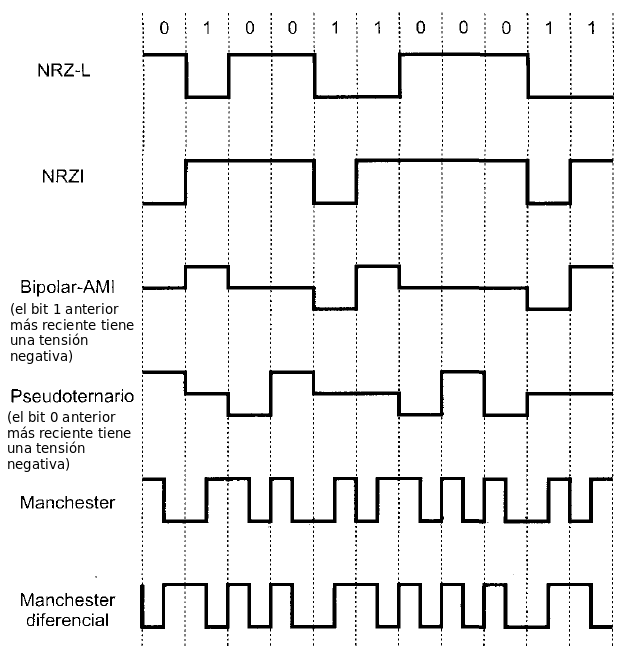
\includegraphics[width=0.8\textwidth-\fboxrule-\fboxrule]{imgs/codificaciones.png}}
\end{figure}

\subsubsection{No Retorno a Cero}
La más simple técnica sería usar un nivel de tensión positivo para representar un 1, y una ausencia de tensión para representar un 0. Las codificaciones NRZ son las más fáciles de implementar, y además hacen un uso eficaz del ancho de banda. Su principal limitación es la presencia de una componente continua y la ausencia de capacidad de sincronización. Dos codificaciones dentro de esta categoría son:
\begin{description}
\item \textbf{NRZ-L} (\textit{nonreturn to zero-level}): usa un nivel negativo para representar un valor binario y una tensión positiva para representar otro. No hay transiciones.
\item \textbf{NRZI} (\textit{nonreturn to zero-level, invert ones}): un 1 se codifica mediante la transición al principio del intervalo de señalización, mientras que un 0 se representa por la ausencia de transmisión.  Una ventaja es que en presencia de ruido es más seguro detectar una transición. Otra ventaja es que se mantiene robusta ante inversiones de polaridad.
\end{description}

\subsubsection{Binario Multinivel}
Usan más de dos niveles de señal.
\begin{description}
\item \textbf{Bipolar-AMI:} el 0 binario se representa por ausencia de señal, y el 1 binario se representa como un pulso positivo o negativo, de forma alternante.
\item \textbf{Pseudoternarios:} como el \textit{bipolar-AMI}, pero invertido: los ceros son los que se alternan.
\end{description}
Estos tipos de esquemas proporcionan una serie de \textbf{ventajas}:
\begin{itemize}
\item Evitan problemas de \textbf{sincronización} en el caso de que haya una cadena larga de unos o ceros (dependiendo de cual se alterna);
\item además, estos últimos no tienen componente de tensión continua, debido a la alternación;
\item el ancho de banda es mucho menor al correspondiente al NRZ;
\item y proporcionan una forma sencilla de detectar errores: cualquier error aislado que elimine/inserte un pulso no cumplirá esta propiedad.
\end{itemize}

Y una serie de \textbf{desventajas}:
\begin{itemize}
\item Problemas de sincronización para cadenas largas de la componente continua.
\item La BER para los códigos NRZ es significativamente menor.
\item La señal puede tomar tres posibles valores, por lo que se necesitan más bits para representar la información.
\item Para obtener la misma probabilidad de error que una NRZ, necesita aproximadamente 3dB más de potencia.
\end{itemize}

\begin{figure}[ht!]
  \caption{Densidad espectral de varios esquemas de codificación.}
  \label{fig:densidad_espectral}  
  \centering
  \hbox{
	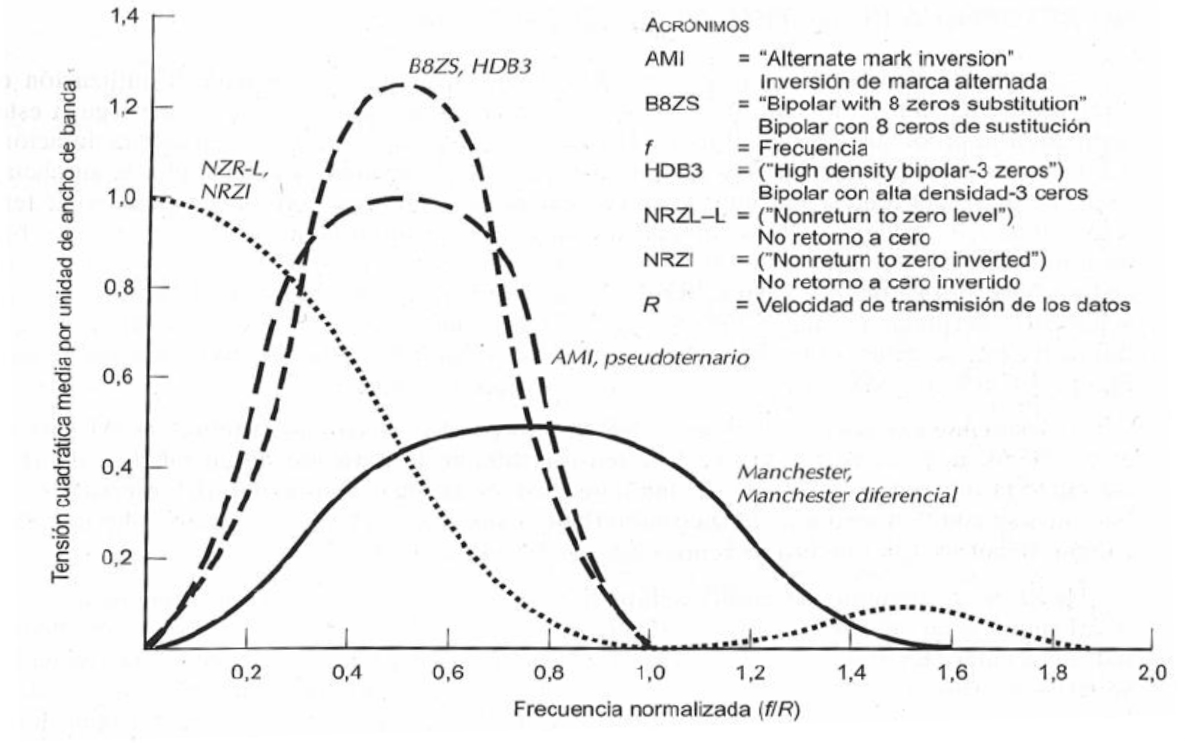
\includegraphics[width=\textwidth-\fboxrule-\fboxrule]{imgs/densidad_espectral.jpg}}
\end{figure}

\subsubsection{Bifase}
Todas las técnicas bifase fuerzan una transición en mitad del intervalo de duración del bit. De esa forma, sirve como procedimiento de sincronización.

\begin{description}
\item \textbf{Manchester:} una transición bajo-alto representa un 1 binario, alto-bajo un 0 binario.
\item \textbf{Manchester diferencial:} la transición se utiliza tan sólo para proporcionar sincronización. La codificación de un 0 se representa por la presencia de una transición al principio del intervalo del bit, y un 1 se representa mediante la ausencia de una transición al principio del intervalo.
\end{description}

La  velocidad de modulación máxima es el doble que en los códigos NRZ; eso significa que el ancho de banda necesario es por tanto mayor. Sin embargo, tienen las siguientes \textbf{ventajas}:
\begin{itemize}
\item \textbf{Sincronización:} la transición que ocurre durante el intervalo de duración de un bit siempre está presente y el receptor puede sincronizar usando dicha transición.
\item \textbf{No tienen componente en continua.}
\item \textbf{Detección de errores:} si se descubre ausencia de transición.
\end{itemize}

\subsubsection{Velocidad de Modulación}

La \textbf{velocidad de transmisión} es $1/T_B$, donde $T_B=$ duración de un bit. La \textbf{velocidad de modulación} es la velocidad a la que se generan los elementos de la señal. En general,
\[D = \frac{R}{L} = \frac{R}{log_2 M},\]
donde:
\begin{enumerate}[ ]
\item $D=$ velocidad de modulación en baudios.
\item $R=$ velocidad de transmisión en bits.
\item $L=$ número de bits por elemento de señal.
\item $M=$ número de elementos de señalización diferentes $=2^L$.
\end{enumerate}

\begin{figure}[ht!]
  \caption{Una cadena de unos a 1 Mbps. \textit{Arriba}, un \textbf{NRZI} (velocidad de modulación de $1/T_B$); \textit{abajo}, codificación \textbf{Manchester} (aquí, la velocidad de modulación es $2/T_B$).}
  \label{fig:vel_modulacion}  
  \centerline{
	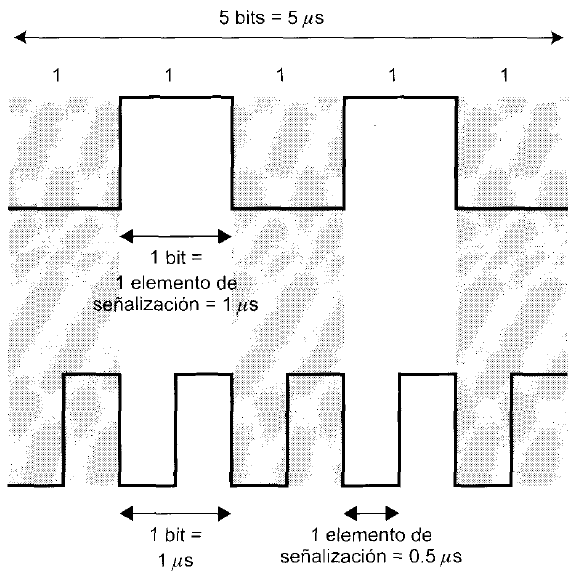
\includegraphics[width=0.6\textwidth-\fboxrule-\fboxrule]{imgs/vel_modulacion.png}}
\end{figure}

\subsubsection{Técnicas de Aleatorización}

Estas técnicas reemplazan las secuencias de bits que den lugar a niveles de tensión constante por otras secuencias que tengan suficiente número de transiciones, de tal manera que el reloj del receptor pueda mantenerse sincronizado. En el receptor se debe identificar la secuencia reemplazada y sustituirla por la secuencia original. Están basadas en la codificación \textbf{bipolar-AMI}.

Tienen como \textbf{objetivos}:
\begin{itemize}
\item Evitar la componente continua.
\item Evitar las secuencias largas que correspondan a niveles de tensión nula.
\item No reducir la velocidad de transmisión de los datos.
\item Tener capacidad de detectar errores.
\end{itemize}

Los dos esquemas de codificación más usuales son:
\begin{description}
\item \textbf{B8ZS} (\textit{Bipolar with 8-Zeros Substitution}): que se realiza según la siguiente regla:
\subitem + Si en la cadena hay un octeto de ceros, y el último valor de tensión anterior a dicho octeto fue:
\subitem a) \textbf{Positivo} $\Rightarrow$ se codifica $000+-0-+$.
\subitem b) \textbf{Negativo} $\Rightarrow$ se codifica $000-+0+-$.

Con este procedimiento se fuerzan dos \textit{violaciones de código}, que son improbables de haber sido causadas por ruido. Por tanto, el receptor identificará dicho patrón y lo interpretará convenientemente como un octeto de ceros.
\item \textbf{HDB3} (\textit{High Density Bipolar-3 zeros}): sustituye cadenas de cuatro ceros por otras con uno o dos pulsos, y al cuarto cero le asigna una \textit{violación de código}. Considera una regla adicional (ver \textbf{figura \ref{fig:hdb3}}) para asegurar que los mismos tengan una polaridad alternante, evitando así la componente continua.
\end{description}

\begin{figure}[ht!]
  \caption{Reglas de sustitución en HDB3.}
  \label{fig:hdb3}  
  \centerline{
	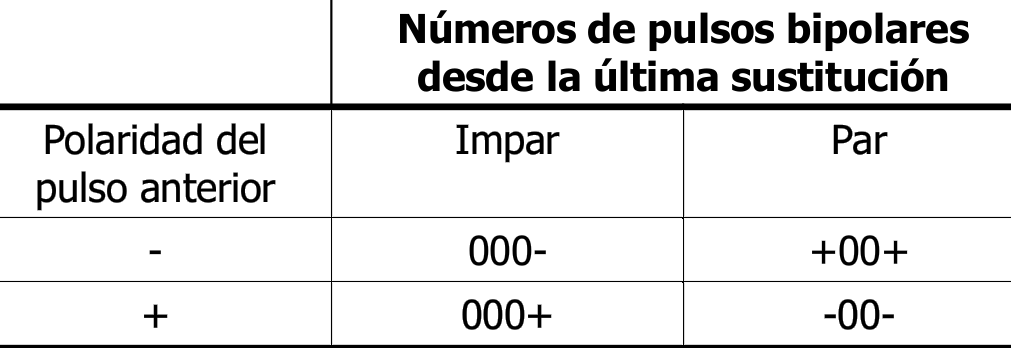
\includegraphics[width=0.5\textwidth-\fboxrule-\fboxrule]{imgs/hdb3.png}}
\end{figure}

Estos códigos son adecuados para la transmisión a altas velocidades.

\begin{figure}[ht!]
  \caption{Reglas de codificación para B8ZS y HDB3.}
  \label{fig:b8zs_hdb3}  
  \centering
  \hbox{
	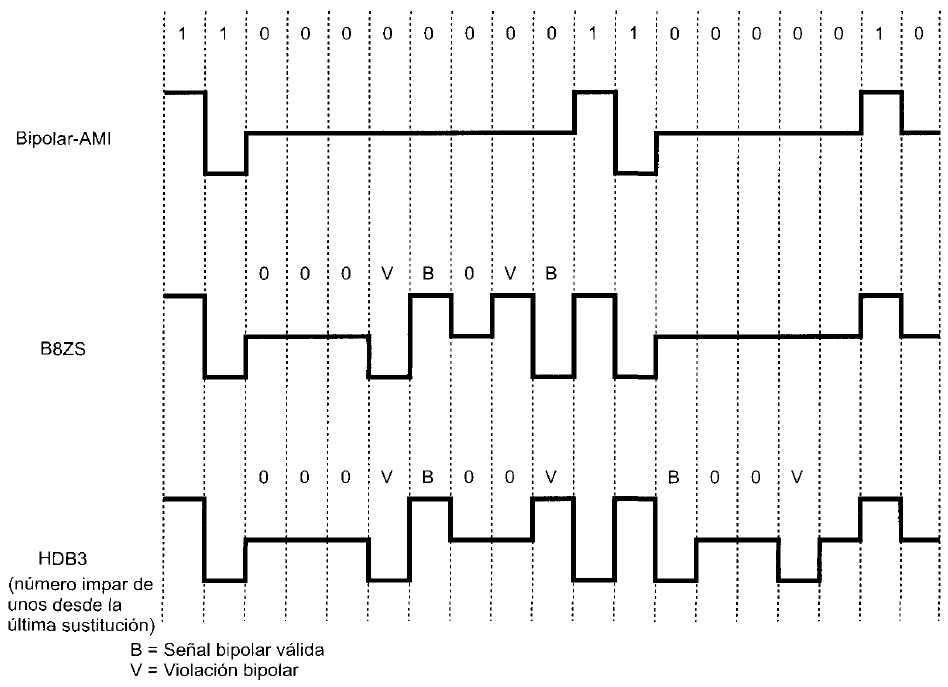
\includegraphics[width=\textwidth-\fboxrule-\fboxrule]{imgs/b8zs_hdb3.png}}
\end{figure}

\subsection{Datos Digitales, Señales Analógicas}

La situación más habitual de transmisión de datos digitales como señales analógicas es a través de la red telefónica. Aunque no es apta para la transmisión de señales digitales, se pueden conectar dispositivos digitales a través de la red mediante el \textit{módem} (modulador-demodulador), el cual convierte los datos digitales en señales analógicas, y viceversa.

\begin{figure}[ht!]
  \caption{Modulación de datos digitales usando señales analógicas.}
  \label{fig:dat_dig_dat_ana}  
  \centerline{
	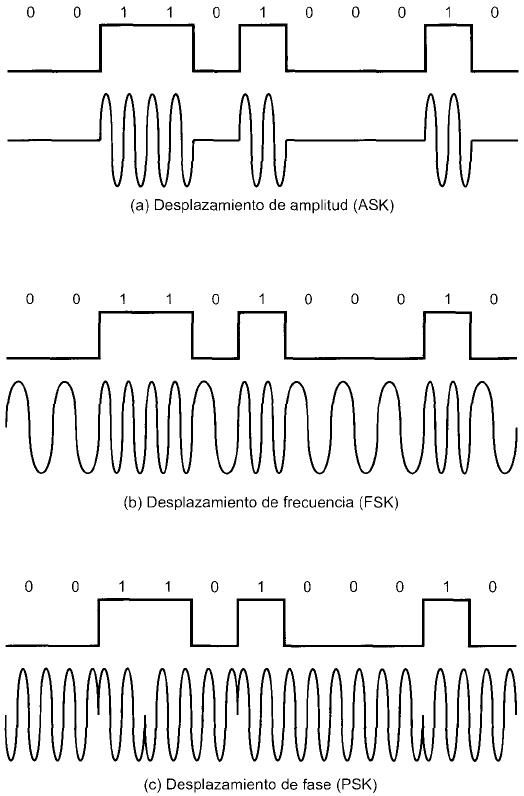
\includegraphics[width=0.6\textwidth-\fboxrule-\fboxrule]{imgs/dat_dig_dat_ana.png}}
\end{figure}

\subsubsection{Modulación por Desplazamiento de Amplitud}
En ASK (\textit{Amplitude-Shift Keying}), los dos valores binarios se representan mediante dos amplitudes diferentes de la portadora. Es usual que una de las amplitudes sea cero. La señal transmitida por cada intevarlo correspondiente a la duración de un bit es:
\[\mathbf{ASK} \qquad
 s(t) = \begin{cases}
        A \cos(2\pi f_c t)  & \text{1 binario,}\\
        0 & \text{0 binario.}
        \end{cases}
\]
Es sensible a cambios repentinos de ganancia, y es bastante ineficaz. Se usa para la transmisión de datos digitales en fibras ópticas.

\subsubsection{Modulación por Desplazamiento de Frecuencia}
El esquema FSK (\textit{Frecuency-Shift Keying}) más habitual es el binario BSFK. En este caso, los dos valores binarios se representan mediante dos frecuencias diferentes, próximas a la frecuencia de la portadora.
\[\mathbf{BFSK} \qquad
 s(t) = \begin{cases}
        A \cos(2\pi f_1 t)  & \text{1 binario,}\\
        A \cos(2\pi f_2 t) & \text{0 binario.}
        \end{cases}
\]
donde $f_1$ y $f_2$ corrresponden a desplazamiento de la frecuencia portadora $f_c$, de igual magnitud, pero en sentidos opuestos.

El BFSK es menos sensible a errores que ASK. Se usa en transmisiones de radio de alta frecuencia.

Una señal más eficaz en el uso del ancho de banda, pero también más susceptible a erroes, es la \textbf{FSK múltiple} (MFSK), en la que se usan más de dos frecuencias. En este caso, cada elemento de señalización representará más de un bit. Se define como:

\[\mathbf{MFSK} \qquad
 s(t) =  A \cos(2\pi f_i t), \quad 1\leq i \leq M
\]
donde:
\begin{enumerate}[ ]
\item $f_i=f_c+(2i - 1 -M)f_d$.
\item $f_c=$ la frecuencia de la portadora.
\item $f_d=$ la diferencia de frecuencias.
\item $L=$ número de bits por elemento de señal.
\item $M=$ número de elementos de señalización diferentes $=2^L$.
\end{enumerate}

\subsubsection{Modulación por Desplazamiento de Fase}
En el esquema PSK (\textit{Phase-Shift Keying}), la fase de la señal portadora se desplaza para representar los datos digitales.

\underline{\textbf{PSK de dos niveles:}}\\
El más simple es el PSK binario, que utiliza dos fases para representar los dígitos binarios.
\[\mathbf{BPSK} \qquad
 s(t) = \begin{cases}
        A \cos(2\pi f_c t) \\
        A \cos(2\pi f_c t + \pi) 
        \end{cases}
      = \begin{cases}
        A \cos(2\pi f_c t)  & \text{1 binario,}\\
        - A \cos(2\pi f_c t) & \text{0 binario.}
        \end{cases}
\]

Una alternativa al BPSK es el \textbf{PSK diferencial} (DPSK, \textit{Differential PSK}). En este esquema, un 0 binario se representa enviando un elemento de señal con la misma fase que el elemento anterior transmitido, y un 1 binario con la fase invertida respecto al anterior elemento transmitido. El desplazamiento de fase es entonces relativo a la fase correspondiente al último símbolo transmitido, en lugar de ser relativo a algún valor constante de referencia.

\begin{figure}[ht!]
  \caption{El PSK diferencial.}
  \label{fig:pskd}  
  \centerline{
	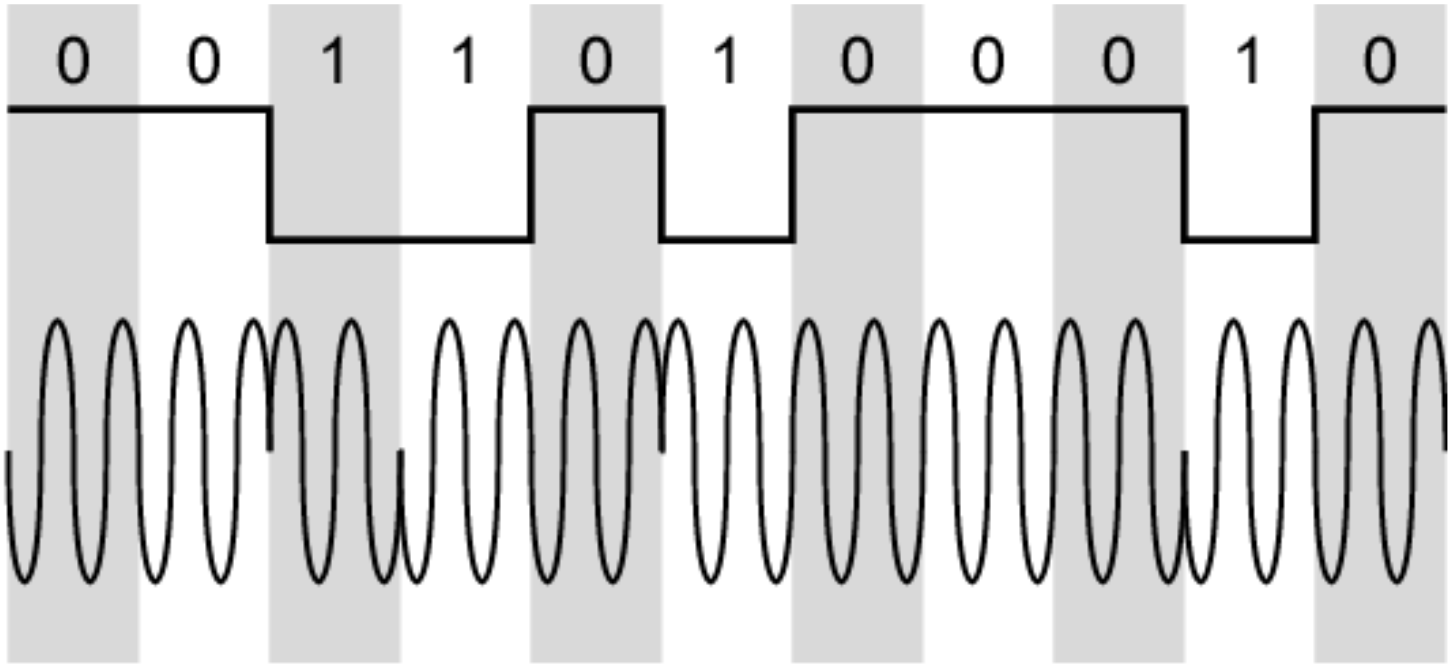
\includegraphics[width=0.5\textwidth-\fboxrule-\fboxrule]{imgs/pskd.png}}
\end{figure}

\underline{\textbf{PSK de cuatro niveles:}}\\
La técnica QPSK (\textit{Quadrature Phase-Shift Keying}) considera desplazamientos múltiplos de $\pi/2$ (90º). Gracias a esto, representamos dos bits en lugar de uno.

\subsubsection{Modulación de Amplitud en Cuadratura}
La técnica QAM (\textit{Quadrature Amplitude Modulation}) es usado en \textit{ADSL} y en algunas técnicas \textit{wireless}. Es una combinación de ASK y PSK. En QAM se aprovecha el hecho de que es posible enviar simultáneamente dos señales diferentes sobre la misma frecuencia portadora, utilizando dos réplicas de la misma, desplazadas entre si 90º. Cada señal portadora se modula usando ASK. Las dos señales independientes se transmiten sobre el mismo medio. Matemáticamente:
\[\mathbf{QAM} \qquad
 s(t) = d_1(t) \cos(2\pi f_c t) + d_2(t) \sin(2\pi f_c t),
\]
donde $d_1$ y $d_2$ son dos secuencias separadas de una señal de entrada binaria $d(t)$.

\small{(\textit{extraído de Wikipedia inglés})} Un \textbf{diagrama de constelación} es una representación de una señal modulada por un esquema digital de modulación tal como el QAM. Muestra a la señal en un diagrama de dispersión en el plano complejo a instantes de elementos de señal. Representa, de forma abstracta, los posibles elementos de señal que pueden ser seleccionados por un cierto esquema de modulación como puntos en el plano complejo. 

\begin{figure}[ht!]
  \caption{Un diagrama de constelación para un QAM-16 rectangular.}
  \label{fig:16qam}  
  \centerline{
	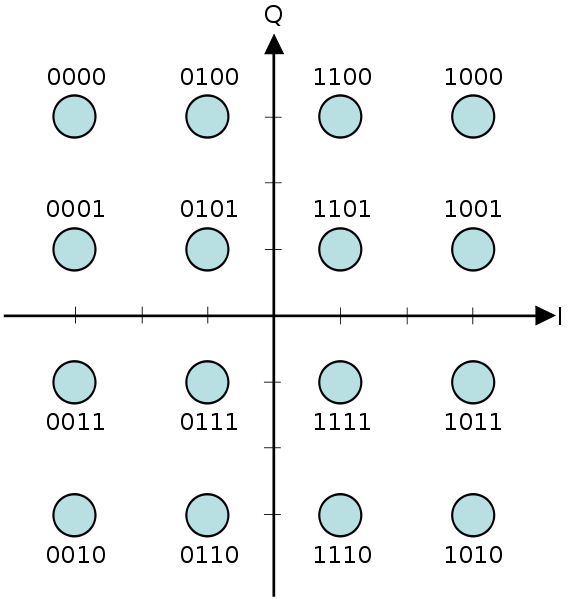
\includegraphics[width=0.5\textwidth-\fboxrule-\fboxrule]{imgs/16qam.png}}
\end{figure}

\subsection{Datos Analógicos, Señales Digitales}

El \textbf{codec} es el dispositivo que se utiliza para la conversión de los datos analógicos en digitales y que, posteriormente, recupera los datos analógicos iniciales a partir de los digitales. Una de las técnicas más importantes usadas en el \textit{codec} es la modulación por pulsos. Dentro de esta categoría tenemos:
\begin{description}
\item \textbf{PWM} (\textit{Pulse Width Modulation}): Cierto valor de amplitud determina, cuando toma la muestra, que ancho va a tener un pulso determinado.
\item \textbf{PPM} (\textit{Pulse Position Modulation}): Dependiendo de donde pongo el pulso en el espacio, va ser el valor de amplitud que tenga la señal.
\item \textbf{PAM} (\textit{Pulse Amplitud Modulation}): Un valor de amplitud ancho, genera un pulso alto, y uno negativo, uno más pequeño. Sufre mucho el ruido.
\item \textbf{PCM} (\textit{Pulse Code Modulation}): Codifica de acuerdo al dato que obtengo.
\end{description}

Obtenemos de esa forma las ventajas (y desventajas) de la \textbf{transmisión digital}.

\pagebreak

\begin{wrapfigure}[14]{r}{.4\textwidth}
  \caption{Modulación de pulsos: (a) señal analógica; (b) pulso de muestreo; (c) PWM; (d) PPM; (e) PAM; (f) PCM.}
  \label{fig:pulsos}  
  \centerline{
	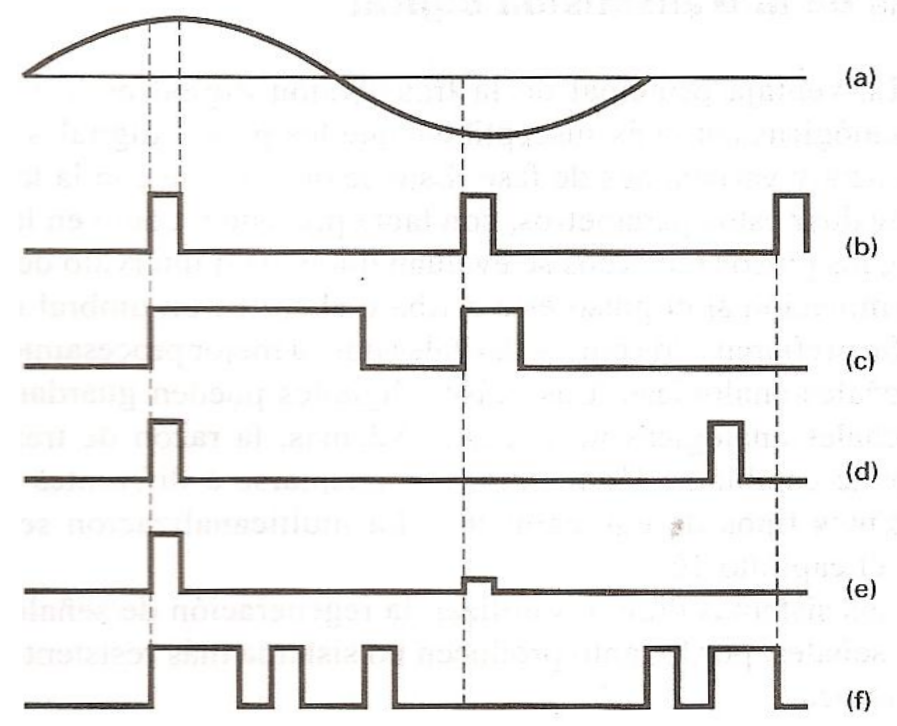
\includegraphics[width=0.4\textwidth-\fboxrule-\fboxrule]{imgs/pulsos.png}}
\end{wrapfigure}

\subsubsection{Pulse Code Modulation}

Se basa en el siguiente teorema:
\begin{quote}
\textbf{Teorema de muestreo:} Si una señal $f(t)$ se muestrea a intervalos regulares de tiempo con una frecuencia mayor que el doble de la frecuencia más alta de la señal original, las muestras así obtenidas contienen toda la información de la señal original. La función $f(t)$ se puede reconstruir a partir de estas muestras mediante la utilización de un filtro paso bajo.
\end{quote}

\underline{\textbf{Características:}}
\begin{itemize}
\item Se utiliza en sistemas de transmisión digital.
\item Son pulsos de longitud fija y amplitud fija.
\item Se usa un sistema binario.
\end{itemize}

El procedimiento consiste en 3 pasos:
\begin{enumerate}
\item \textbf{Muestreo:} Respetando el teorema, tomamos muestras \textit{analógicas} llamadas muestras PAM.
\item \textbf{Cuantización:} Permite aproximar la muestra
a uno de los niveles de escala designada. Al cuantizar la señal analógica, pierdo información y por lo tanto pierdo el valor real de la señal. Decimos entonces que se introduce un error de cuantización de la señal, dado por:
\[\text{SNR}_\text{dB} = 20 \log 2^n + 1.76 \text{ dB} = 6.02n + 1.76 \text{ dB}.\]
De aquí, que cada bit adicional que se use aumentará la SNR en 6dB.
\item \textbf{Codificación:} Para convertir las muestras PAM a digital, a cada una de ellas se les debe asignar un código binario. Si las muestras son de $n$ bits, habrá $2^n$ niveles de cuantización posibles.
\end{enumerate}

Hasta acá obtuvimos una señal digital que consiste en boques de $n$ bits donde cada uno corresponde a la amplitud de un impulso PCM.

\textit{Ejemplo}: Sabiendo que los datos de voz se limitan a frecuencias por debajo de los 4000hz, supongamos que tenemos una señal de voz. Usando muestras de 8 bits, permite $2^8 = 256$ niveles de cuantización, esto implica que para una única señal de voz se necesitan 8000hz, o lo que es lo mismo, 8000 muestras $\times$ 8 bits $= 64$ kbps.

\end{document}